\documentclass[french]{article}
 
\usepackage[utf8]{inputenc}
\usepackage[T1]{fontenc}
\usepackage{babel}
\usepackage[pdftex]{graphicx}
\usepackage{appendix}
\usepackage{float}
\DeclareUnicodeCharacter{2212}{-}
\DeclareUnicodeCharacter{0301}{'}

% Mode paysage pour le Gantt
\usepackage{pdflscape}
\usepackage{rotating}
\usepackage[dvipsnames]{xcolor}
\definecolor{ganttBlue}{rgb}{0.4, 0.5, 1.0}
\definecolor{ganttGreen}{rgb}{0.4, 0.8, 0.0}
\definecolor{ganttOrange}{rgb}{1.0, 0.48, 0.2}

\usepackage{biblatex}
\addbibresource{biblio.bib}

\usepackage[colorlinks=true,linkcolor=black,urlcolor=blue]{hyperref}

\newcommand{\HRule}{\rule{\linewidth}{0.5mm}}
\newcommand{\itembf}[1]{\item \textbf{#1}\\}

\begin{document}
% PAGE DE GARDE
\begin{titlepage}
  \begin{sffamily}
  \begin{center}

    \textsc{\LARGE Projet de programmation}\\[2cm]

    \textsc{\Large Cahier des besoins}\\[1.5cm]

    % Title
    \HRule \\[0.4cm]
    { \huge \bfseries Environnement d'exécution y86+HCL\\[0.4cm] }

    \HRule \\[1cm]
    
\includegraphics[scale=0.07]{img/logoUB.jpg}
    \\[2cm]

    % Auteurs à gauche
    \begin{minipage}{0.4\textwidth}
      \begin{flushleft} \large
        \textsc{BANDET} Alexis\\
        \textsc{GAISSET} Valentin\\
        \textsc{GUISSET} Romain\\
        \textsc{SIMBA} Florian\\
      \end{flushleft}
    \end{minipage}
    % professeur à droite
    \begin{minipage}{0.4\textwidth}
      \begin{flushright} \large
        \emph{\underline{Professeur} :}\\ Mme. \textsc{ZANON-BOITO} Francieli\\
      \end{flushright}
    \end{minipage}

    \vfill

    % Date en bas de page
    {\large Janvier 2019}

  \end{center}
  \end{sffamily}
\end{titlepage}

\tableofcontents
\newpage

\section{Introduction}
% Rappel du projet, des clients, des tenants et aboutissants

Le projet \textbf{Environnement d'exécution y86+HCL} a pour but d'améliorer un simulateur déjà existant de ce dit environnement. \\

Le \textbf{y86} est une simplification de l'architecture x86 et a été créé à des fins pédagogiques, pour permettre à des étudiants d'appréhender l'architecture des processeurs en faisant abstraction de détails complexes. \\
Il a été créé par R. E. Bryant et D. R. O'Hallaron, deux professeurs de la \textit{Carnegie Mellon University}. \\

Les outils \cite{standalone-app} fournis par ces deux enseignants se font vieux et peu pratiques à utiliser, surtout pour des débutants qui ne sont pas forcément à l'aise avec la compilation en C. Pour palier à ce soucis, différentes applications web ont déjà été développé, plus ou moins complètes, plus ou moins modulaires, etc. De part sa conception il contient une double dépendance lors de la modification du jeu d'instruction, ce qui oblige la modification de plusieurs fichiers lors de l'ajout ou de la modification d'une instruction du processeur. Le processus de modification de \textit{l'instruction set} est alors en parti dénaturé et se transforme en compréhension de la compilation du programme.\\
% Rajouter des annotations vers la webographie pour le projet x86 et les différentes webapp

Nos clients, \textbf{Aurélien ESNARD} et \textbf{François PELLEGRINI} ont donc proposé ce projet dans le but d'améliorer l'environnement de travail des futurs étudiants. Plusieurs objectifs sont de mise, à savoir : 

\begin{itemize}
    \item Une \textbf{interface intuitive} et agréable.
    \item Gestion du \textbf{HCL} (\textbf{H}ardware \textbf{C}ontrol \textbf{L}anguage) afin de :
    \begin{itemize}
        \item Modifier des instructions existantes
        \item Créer de nouvelles instructions
    \end{itemize}{}
    \item Avoir une vue détaillée de l'\textbf{état du processeur} (stages).
    \item L'application doit être  exécutée sur plusieurs système d'exploitation.
    \item L'application doit être \textbf{accessible au plus grand nombre}, notamment aux personnes soufrant d'un handicap.
    \item L'application doit être \textbf{modulaire} et \textbf{documentée} afin de simplifier l'ajout de fonctionnalités ultérieurement. Cela doit notamment permettre l'implémentation de différentes versions du simulateur (\textit{sequential, pipelined}).
\end{itemize}

\section{Mise en contexte}
\label{contexte}

La suite du document traitera d'éléments liés au y86. Afin d'en faciliter la compréhension, nous allons expliquer ici quelques une de ces notions.

\begin{enumerate}
    \item Fichiers \textbf{.ys} :\\
    Fichier source contenant le code y86 à compiler.
    \begin{figure}[H]
        \centering
        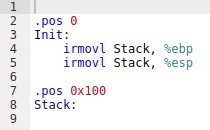
\includegraphics{img/ex_ys.png}
        \caption{Code d'un programme y86 (.ys)}
        \label{fig:ex_yo}
    \end{figure}
    
    \item Fichiers \textbf{.yo} :\\
    Fichier objet contenant le code compilé à partir du .ys source.\\
    \begin{figure}[H]
        \centering
        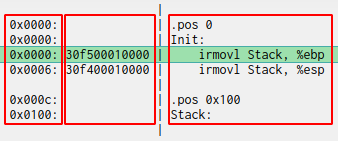
\includegraphics{img/ex_yo.png}
        \caption{fichier object (.yo) généré à partir d'un code source (.ys)}
        \label{fig:ex_yo}
    \end{figure}
    De gauche à droite, pour chaque ligne :
    \begin{enumerate}
        \item L'adresse de l'instruction (en hexadécimal)
        \item Le codage de l'instruction (en hexadécimal)
        \item L'instruction même, telle qu'elle est dans le code source
    \end{enumerate}
    
    \item \textbf{.hcl} :\\
    Fichier décrivant le comportement du processeur face à une instruction.\\
    \begin{figure}[H]
        \centering
        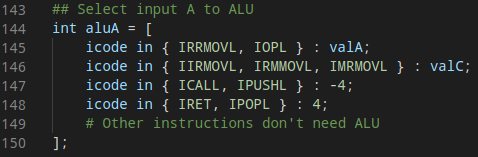
\includegraphics{img/ex_hcl.png}
        \caption{Exemple de code HCL}
        \label{fig:ex_hcl}
    \end{figure}
    Dans cet exemple, si l'instruction est IRRMOVL, alors valA sera mise dans aluA. Le code HCL est ensuite compilé dans le langage utilisé par le simulateur. De cette manière, la simulation pourra appeler les fonctions générées et ainsi savoir comment traiter chaque instruction.
\end{enumerate}

\section{État de l'art}
% Etat actuel du projet

\subsection{Application web \cite{webapp-ub}}

Actuellement, la modification de quelques fichiers du simulateur web est nécessaire pour ajouter ou modifier une instruction :
\begin{itemize}
    \item \textbf{ace/mode-y86.js} qui contient les expression régulières acceptés par le compilateur.
    \item \textbf{assem.js} qui contient les fonctions nécessaire pour effectuer la conversion du code assembleur en code binaire.
    \item \textbf{general.js} qui contient les listes d'instructions avec leurs codages (\textit{icode \& ifun}).
    \item \textbf{syntax.js} qui contient une liste de toutes les syntaxes possibles.
    \item \textbf{instr.js} qui contient un tableau avec les actions de chaque instruction. Ce fichier pourra nous être utile pour récupérer l'état du processeur pour chaque étage au cas par cas). \\
\end{itemize}

Nous sommes entrain de réfléchir comment bien prendre en compte les modifications de l'utilisateur tout en gardant le sens pédagogique de l'outil avec un code flexible et modulaire.

\subsection{Application x86 (standalone)}

Cette application est le programme originel permettant de simuler un processeur y86 ainsi que sa mémoire. Elle a été créée par les professeurs R. E. Bryant et D. R. O'Hallaron, de la Carnegie Mellon University. \\
Elle propose un mode graphique (Tcl/Tk) ainsi qu'un mode textuel pour une utilisation depuis un terminal. Le comportement du processeur face aux instructions peut être modifié en utilisant le langage HCL. Ce fichier HCL est converti en fichier source C, compilé, puis lié au simulateur durant la phase d'édition de lien. Chaque modification de ce fichier nécessite donc de recompiler le simulateur (ou à minima de ré-effectuer l'édition de liens).

Plus d'informations à propos de cette application sont disponibles sur le wiki du GitLab \cite{wiki-application-y86}.

\section{Description des besoins}

Nous présenterons ci-dessous les différents besoins auxquels devra répondre l'application développée. Du fait que nous partirons très probablement d'une application déjà existante, certains besoins seront donc déjà implémentés.

Une des principales contraintes étant la facilité d'accès pour les étudiants et la portabilité, les besoins seront décrits dans l'optique du développement d'une application web.

\newpage
\subsection{Besoins fonctionnels}
% Liste des besoins
Fonctionnalités de l'application :

\begin{enumerate}
    \itembf{Saisie du code y86}
    \begin{enumerate}
        \itembf{Éditeur de code y86} 
            Il doit respecter les contraintes suivantes :
        \begin{enumerate}
            \itembf{Saisir du code (y86 uniquement)}
            \itembf{Afficher les numéros de lignes}
            \itembf{Colorer syntaxiquement le texte saisi}
            La coloration doit permettre de distinguer les différents éléments du langage, à savoir :
            \begin{itemize}
                \item Les instructions en bleu foncé
                \item Les constantes en rouge
                \item Les labels en noir
                \item Les registres en bleu clair
                \item Les commentaires en vert
            \end{itemize}
            \itembf{Analyser statiquement le code afin d'aider à son écriture}
            Si jamais le code saisi n'est pas valide, une croix rouge doit apparaître à gauche de l'éditeur. Si la souris est au dessus de cette croix, l'erreur doit être affichée. \\
            L'analyse statique (ainsi que la coloration syntaxique) devront s'adapter à l'ajout / modification d'instructions. Voir \ref{personnalisation_simulateur} pour plus de détails.
        \end{enumerate}{}
        \begin{figure}[H]
            \centering
            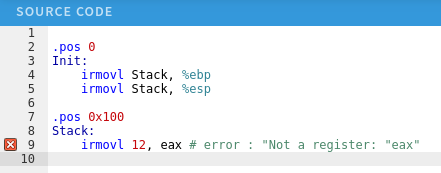
\includegraphics{img/ex_ys_erreur.png}
            \caption{Éditeur de code y86 utilisant l'analyse statique de code}
            \label{fig:ex_ys_erreur}
        \end{figure}
        
        \itembf{Charger un fichier de code y86 \textbf{.ys}}
        Bouton pour charger un fichier \textbf{.ys} depuis l'ordinateur de l'utilisateur. Le contenu de ce fichier est ensuite mis dans l'\textbf{éditeur de code y86} décrit précédemment.
    \end{enumerate}{}
    
    
    \itembf{Compilation}
    L'application doit être capable de générer du code objet (\textbf{.yo}) à partir du code présent dans l'\textbf{éditeur de code y86}.\\
    Attention cependant, le compilateur y86 devra pouvoir s'adapter à l'ajout / modification d'instruction. Se référer au besoin \textbf{Personnalisation du simulateur} pour ça (voir \ref{personnalisation_simulateur}). 
    Les contraintes suivantes doivent être respectées :
    \begin{enumerate}
        \itembf{Bouton de compilation}
        Il permet de lancer la compilation de \textbf{ys} vers \textbf{yo}. Le code source est récupéré dans le fenêtre d'édition de code.
        \itembf{Affichage du code objet généré}
        Une fenêtre doit afficher le code \textbf{.yo} généré. L'affichage du code objet doit respecter le format des fichiers \textbf{.yo}. Un exemple est disponible dans la partie de mise en contexte (voir \ref{contexte}).
        \itembf{Gestion des erreurs de compilation}
        Si le code en entrée n'est pas valide, l'erreur de compilation doit être affichée, en rouge, ainsi que la ligne incriminée.
        \begin{figure}[H]
            \centering
            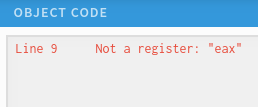
\includegraphics[]{img/ex_erreur_compilation.png}
            \caption{La fenêtre du code objet affiche l'erreur en rouge}
            \label{fig:ex_erreur_compilation}
        \end{figure}
    \end{enumerate}{}
    
    
    \itembf{Exécution}
    Si du code objet est présent (dans la fenêtre de compilation vue précédemment), l'utilisateur doit pouvoir exécuter ce code, d'une traite ou étape par étape, et doit pouvoir voir les valeurs contenues dans les registres, dans la mémoire ainsi que les drapeaux de conditions. Cela correspond à l'état de la machine. Parallèlement à ça, l'état du processeur doit aussi être visible, c'est à dire les valeurs contenues dans les différents registres du processeur après l'exécution d'une instruction.\\ 

    Voici les besoins détaillés :
    \begin{enumerate}
            \itembf{Affichage de l'état de la machine}
            \begin{enumerate}
                \itembf{Affichage des registres}
                Les registres de \%eax à \%edi (nom, valeur en base 8, valeur en base 10)\\
                Exemple : \textbf{\%eax 0x00000100 256}
                \itembf{Affichage des drapeaux de condition}
                Ces drapeaux sont utilisés pour savoir si des "jumps" seront effectués. Ils sont de la forme (nom, valeur en base 10)\\
                Exemple : \textbf{SF 0}
                \itembf{Le statut du processeur}
                Il permet de voir le statut à proprement parlé (OK, HALT) ainsi que le compteur d'instruction, qui contient l'adresse de la prochaine instruction à exécuter.
            \end{enumerate}{}
            \begin{figure}[H]
                \centering
                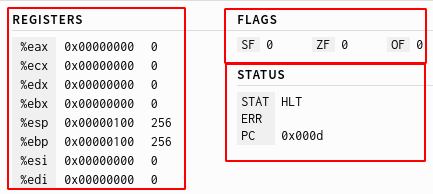
\includegraphics{img/ex_vue_registres.png}
                \caption{Registres du processeur}
                \label{fig:ex_vue_registres}
            \end{figure}
            
            \itembf{Affichage de l'état du processeur}
            Affiche les différents \textit{stages} du processeur, à savoir \textbf{Fetch}, \textbf{Decode / Read}, \textbf{Execute}, \textbf{Memory} et \textbf{PC update} en séquentiel.\\
            Chaque \textit{stage} affiche une ou plusieurs valeur. Ces valeurs peuvent être de forme textuelle, ou bien numérique.\\
            Cette fenêtre est mise à jour après chaque exécution d'une instruction.
            \begin{figure}[H]
                \centering
                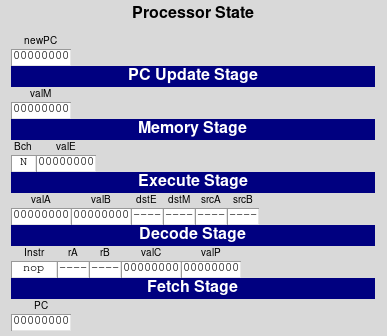
\includegraphics{img/ex_statut_proc.png}
                \caption{Vue des différents \textit{stages} du processeur}
                \label{fig:ex_statut_proc}
            \end{figure}
            
            \itembf{Aide à la visualisation des accès mémoire}
            La mémoire utilisée par le processeur est affichée sous forme de liste. On peut y voir l'adresse ainsi que le contenu.
            \begin{figure}[H]
                \centering
                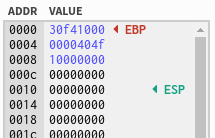
\includegraphics{img/ex_memoire.png}
                \caption{Affichage de la mémoire. On peut y voir les valeurs des registres \%ebp et \%esp ainsi que les cases accédées (en bleu)}
                \label{fig:ex_memoire}
            \end{figure}
            Lorsqu'un accès mémoire sera effectué, l'utilisateur devra en être notifié (par exemple saut sur la case concernée, pointée par une flèche ou mise en surbrillance). Cela à pour but de permettre à l'étudiant de facilement visualiser l'impact de son code sur la mémoire.Q
    \end{enumerate}{}

    \itembf{Personnalisation du simulateur}
    \label{personnalisation_simulateur}
    Le simulateur a pour principale contrainte d'être personalisable. Son comportement devra pouvoir être changé de manière relativement aisée. Par exemple, on pourrait souhaiter implémenter une version \textit{pipelined} du processeur, en plus de la version \textit{sequential} de base.\\
    Un autre but pédagogique consiste à permettre aux élèves d'insérer / modifier des instructions. 
    Afin de se représenter les dépendances entre les différents modules (HCL, yas, ISA, simulateur, etc...), un diagramme disponible en annexe \ref{fig:diag_archi_modulaire_standalone} montre une potentielle esquisse d'architecture, ainsi que les dépendances entre les différents composants.
    
    \begin{enumerate}
        \itembf{Personnalisation des instructions}
        \begin{enumerate}
            \itembf{Éditeur d'instructions}
            C'est depuis cet éditeur que l'on ajoutera / supprimera / modifiera une instruction. Cet éditeur a plusieurs objectifs. Premièrement, vérifier que le nombre de couple (icode, ifun) n'est jamais dupliqué et qu'il n'y a pas plus de 16 instructions. Dans un second temps, il doit faciliter la vie des étudiants en simplifiant la saisie de nouvelles instructions.
            \begin{figure}[H]
                \centering
                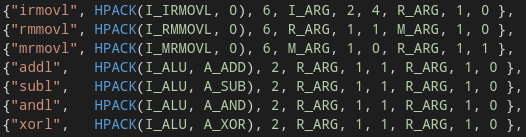
\includegraphics{img/ex_ancien_is.png}
                \caption{Codage d'une instruction dans la version x86. De gauche à doite, l'identifiant, le couple (icode, ifun), la taille en octets de l'instruction, le type du premier argument (constante / registre / adresse mémoire), la position du premier argument une fois l'instruction encodée, la taille en octets du premier argument, le type du second argument, la position du second argument une fois l'instruction encodée, la taille en octets du second argument}
                \label{fig:ex_ancien_is}
            \end{figure}
            Une version plus visuelle est donc attendue afin de limiter les erreur en abstrayant le codage.
            
            \itembf{Utilisation du HCL}
            Le HCL est le code à éditer pour indiquer comment traiter une instruction. Une fois le code HCL saisi, il faudra le compiler en JavaScript afin que le simulateur puisse y accéder. Ce besoin requiert donc :
            \begin{enumerate}
                \itembf{Éditeur de HCL}
                Cet éditeur permettra de saisir du code HCL. A l'image de l'éditeur de code y86, l'analyse statique de code ainsi que la coloration syntaxique propre au HCL serait souhaitable.
                
                \itembf{Bouton de compilation}
                Ce bouton convertit le code HCL présent dans l'éditeur en code JavaScript qui pourra être appelé par le simulateur. 
                
                \itembf{Fenêtre de visualisation de résultat}
                Adjacente à l'éditeur de code HCL, cette fenêtre devra afficher le code JavaScript généré à partir du HCL. A l'instar de la fenêtre de compilation du y86, les erreurs de compilation devront y être affichées en rouge si il en existe.
            \end{enumerate}
        \end{enumerate}
    \end{enumerate}
\end{enumerate}


\subsection{Besoins non fonctionnels}
% Liste des besoins
\begin{enumerate}
    \itembf{Interface multilingue}\\
    Nous allons devoir utiliser des fichiers de \textit{strings.xml} pour afficher le texte de l'interface. Cela permet, dès le début de la conception de l'application, de supporter toute les langues. Cependant nous allons uniquement implémenter l'anglais, l'objectif de ce besoin est simplement de proposer une modularité de plus au niveau de l'interface.
    \\
    \itembf{Automatisation des tâches}\label{Besoin nf Automatisation des tâches}\\
    Une fonctionnalité souhaitée est l'automatisation de certaines tâches, notamment pour les correcteurs. L'idée serait de faire des requêtes paramétrées qui retourneraient un résultat. A ce jour, la principale utilisation serait la récupération d'un dump de l'état de la machine après exécution d'un programme, avec un HCL et un IS donné, afin de voir avec quel registre / "case mémoire" le programme interagit.
    \\\\
    \underline{Exemple :}\\ \textbf{wget} <hostname>?file=test.y86\&hcl=student.hcl\&conf=student.json\\\&action=memorydump\&breakline=10
    \\\\
    Ce système implique une certaine vigilance lors de la phase de conception de l'application. En effet, la requête paramétrée étant reçue par le serveur, ce sera à lui de la traiter. Si le code du simulateur est exécuté seulement du côté du client, il faut penser à un moyen de traitement autonome pour le serveur. Plusieurs pistes sont bien évidemment envisageables. Ces dites pistes seront abordées dans un autre document que celui-ci.
    \\
    \itembf{Simulateur y86}
    Il s'agit du module qui exécutera les instructions contenues dans le .yo en simulant le processeur. Il appellera les fonctions fournies par le script généré à partir du HCL. A priori, ce module ne sera pas modifiable par l'utilisateur, mais seulement par les développeurs. \\
    \\
    \itembf{Accessibilité}
    L’application devra être ouverte au personnes souffrant d’un trouble de la vision. La pensée principale vient aux personnes atteinte de cécité totale pour qui les outils actuels ne sont pas adaptés. Pour cela le document de référence de l’administration française\footnote{Référentiel Général d'Accessibilité pour les Administrations (RGAA)} peut être d’une grande aide, ainsi que le recours à un spécialiste de la question, comme M. Samuel THIBAULT.

\end{enumerate}

\subsection{Classement des besoins par ordre de priorité}
Dans l'intérêt de mener à bien ce projet, nous classerons les besoins selon leur priorité afin de ne pas disperser nos efforts. 

nous garderons le simulateur actuel mais en y ajoutant :
\begin{itemize}
    \item État du processeur
    \item Personnalisation du simulateur (Ajout d'instructions)
    \item Automatisation des tâches
    \item Interface multilingue
    \item Aide à la visualisation des accès mémoire
\end{itemize}


\subsection{Changements des besoins}\label{Changements des besoins}
\begin{enumerate}
    \itembf{Automatisation des tâches}
    Ce besoin nous a été exprimé sous la forme décrite en section \ref{Besoin nf Automatisation des tâches}. Cela requiert un \textit{back-end} qui traiterait ce type de requête, or l'application que nous allons développer est uniquement constituée d'un \textit{front-end}. Le besoin risque donc de changer.
\end{enumerate}
    
\subsection{L'interface utilisateur}

L'interface utilisateur telle que prototypée propose de mettre en place un système d'onglets et de boutons afin d'interagir avec l'utilisateur. Pour cela les trois ou quatre modes seront représentés par un onglet chacun. Le mode \textit{Instruction set}, permettant l'ajout d'instruction, pourrait être intégré au mode \textit{HCL} par la suite si cela permet une meilleure ergonomie. 

Chaque onglet posséderait des interfaces différentes: 

\begin{itemize}
    \item \textbf{Éditeur} : Possède un éditeur de texte pour modifier les fichier .ys, une fenêtre d'exécution où l'utilisateur peut observer les instructions s'exécuter étape par étape (step-by-step) et un dump de la mémoire.
    Il peut aussi posséder les clés pour exécuter le programme tel que le boutons "Step" ou "Assemble". Ces derniers pourrons tout aussi bien être global (commun à tous les onglets). C'est une décision qui devra être prise en fonction des résultats de l'expérimentation.
    
    \item \textbf{HCL} : Le mode qui regroupe les fonctionnalités nécessaires au bon développement du HCL par l'utilisateur. Cette interface regroupe un éditeur de texte pour éditer le HCL et la vu des différents états du processeurs (Stages) à chaque instruction.
    
    \item \textbf{Mode avancé} : Cette vue proposée par le client permet de visualiser en parallèle le code qui s'exécute comme dans le mode Éditeur et le Stages du processeur comme dans le mode HCL. L'intérêt principal de ce mode est de permettre à l'utilisateur de comprendre ce qu'il se passe dans le processeur à chaque instruction.\\
\end{itemize}

L'ergonomie primera sur le choix finale de l'interface. Cette dernière doit cependant permettre de :

\begin{itemize}
    \item visualiser l'état du processeur comme décrite figure \ref{fig:ex_statut_proc}.
    \item visualiser l'état de la mémoire.
    \item éditer le fichier .hcl et .ys
    \item visualiser l'état des registres et des flags.\\
\end{itemize}

Outre ces éléments de visualisation, l'interface doit aussi permettre de compiler et d'exécuter le programme. Soit d'un coup, soit étape par étape. Une fonction pour revenir au début de l'exécution (Reset) et une pour sauvegarder ou charger un fichier hcl ou ys extérieur sont aussi souhaitées.

En revanche, la possibilité de faire des breakpoints, bien que pratique, ne fait pas parti des besoins fonctionnels. L'accessibilité aux utilisateurs atteint de troubles visuelles ne doit pas obligatoirement se faire via cette interface.

\newpage
\begin{figure}
    \centering
    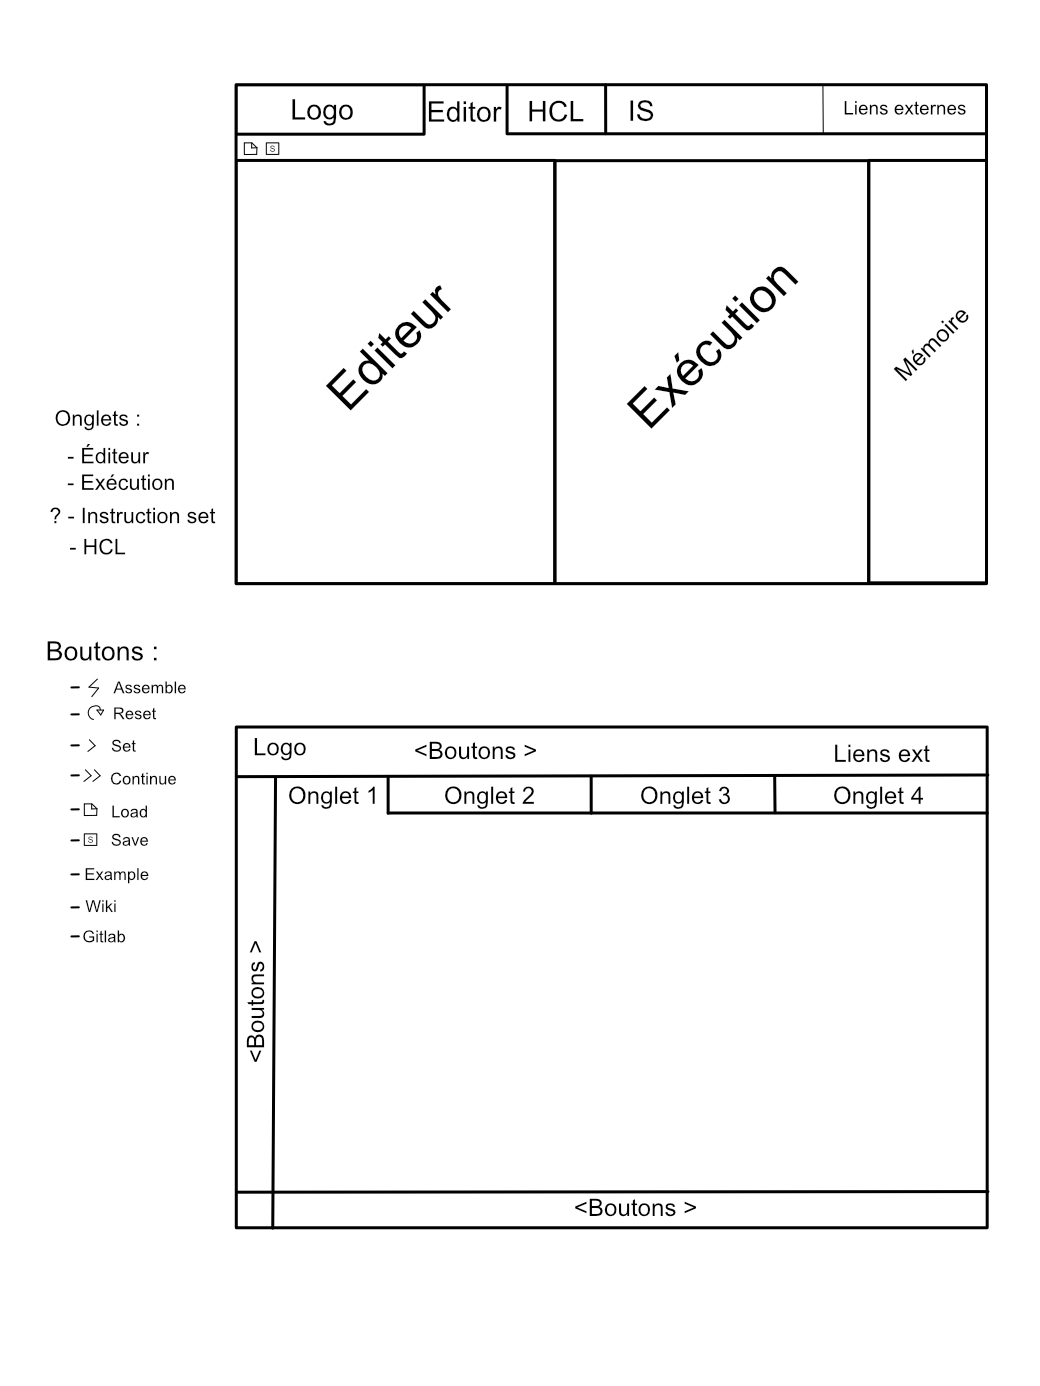
\includegraphics[scale=0.35]{img/croquis_interface.jpg}
    \caption{Prototypes de l'interface utilisateur}
    \label{fig:my_label}
\end{figure}

\newpage
\begin{landscape}
    \section{Planification des tâches}
    \begin{figure}[H]
        \centering
        \rotatebox{90}{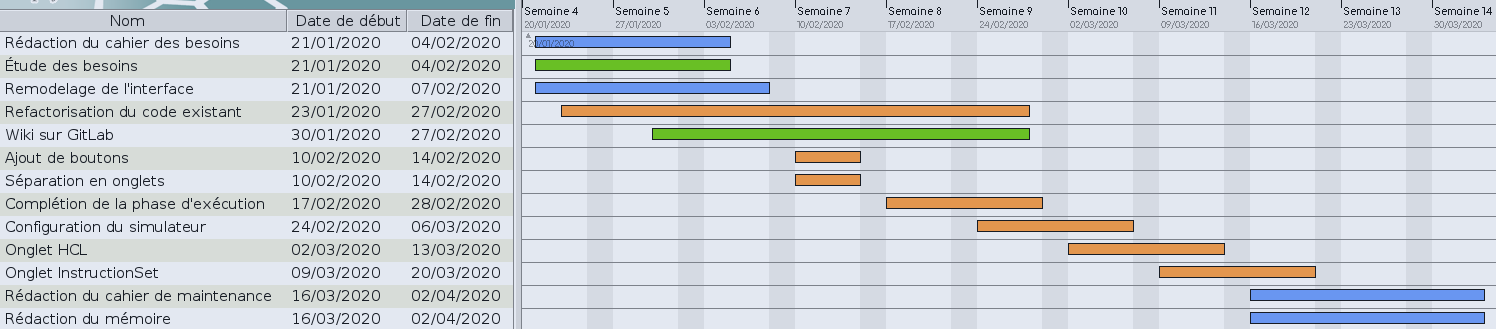
\includegraphics[width=\paperwidth,angle=-90]{img/gantt.png}}
        \caption{Diagramme de Gantt}
        \label{fig:gantt}
    \end{figure}
    \textbf{Légende :}
    \\
    \begin{itemize}
        \item[] \colorbox{ganttBlue}{\color{ganttBlue}{ - }} Rédaction de documents
        \\
        \item[] \colorbox{ganttGreen}{\color{ganttGreen}{ - }} Travail de recherches
        \\
        \item[] \colorbox{ganttOrange}{\color{ganttOrange}{ - }} Développment
    \end{itemize}
    \bigskip
    \hspace{\parindent} Nous avons choisit de ne pas assigner les tâches à des membres du projet, car ce projet implique une importante phase d'étude des besoins. Suivit d'une phase de développement entièrement basée sur la précédente. Or certains besoins sont voués à changer car ils dépendent entre autre de la réalisation préalable d'autre besoins (voir la section \ref{Changements des besoins}).
\end{landscape}

\printbibliography

\section{Annexes}

\begin{appendix}

\begin{figure}[H]
    \centering
    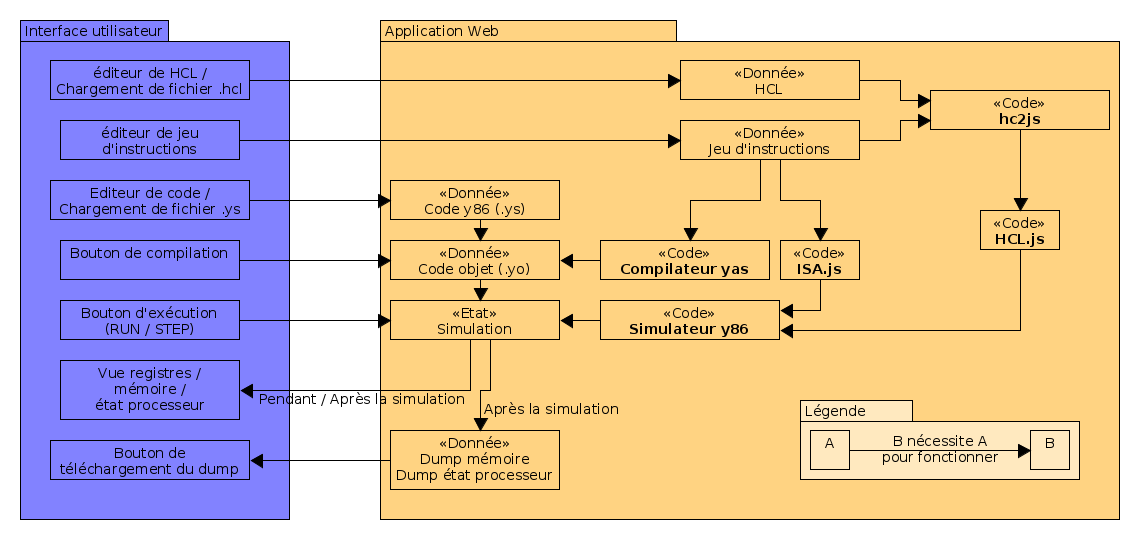
\includegraphics[width=\paperwidth, angle=270]{img/architecture_modulaire_standalone.png}
    \caption{Potentielle architecture pour une application web standalone}
    \label{fig:diag_archi_modulaire_standalone}
\end{figure}

\subsection{Description de l'architecture}

L'architecture affichée précédemment montre les différents composants ainsi que les inter-dépendances, symbolisées par des flèches. Ainsi, on peut clairement voir les modules "directeurs" de l'application. Par exemple, on peut remarquer que l'édition du jeu d'instruction sera essentielle pour compiler du code y86, permettre au simulateur de s'exécuter et compiler le HCL.js. Cette séparation des différents composants a pour objectif de simplifier le principe de modularité en réduisant le couplage au maximum.

\end{appendix}

\end{document}
